\documentclass{article}
\usepackage[utf8]{inputenc}
\usepackage{graphicx}
\usepackage{subfigure}
\usepackage{caption}


\title{Sample Report}
\author{Pranit Zope AE20B046}
\date{17 August 2021}

\begin{document}

\maketitle
This is my first report being produced on \LaTeX. 

\section{Graphical Representation of Equations}
This section shows us a 2-Dimensional and a 3-dimesional graph and explains a bit about it. These were created using Numpy and Matplotlib.
\subsection{2D Graph}

\begin{figure}[!h]
\centering
\subfigure[$y = x^3-x^2-2x$]{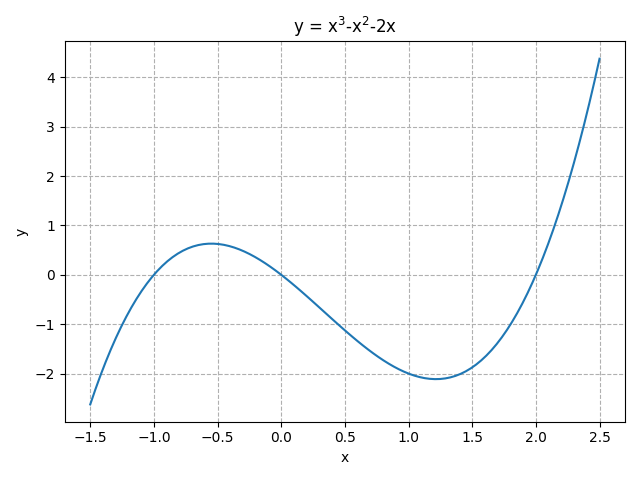
\includegraphics[width=0.6\columnwidth]{2dgraph.png}\label{fig:graph1}}
\label{fig:graphs}
\end{figure}


Figure ~\ref{fig:graph1} shows the equation of the curve:
\begin{equation}y = x^3-x^2-2x\end{equation}
This is a cubic polynomial with 3 real roots. When Factorised, this equation gives us the roots : $2,0$ and $-1$, clearly shown in the figure. From this figure, we also can figure out that the maxima of the function is somewhere around $x=-0.5$ and the minima is somewhere between $x=1$ and $x=1.5$
\pagebreak

\subsection{3D Graph}
Here, apart from numpy and matplotlib, we also have used mplot3d from matplotlib toolkit for plotting the 3D curve.

\begin{figure}[!ht]
\centering
\subfigure[$z = sin(2x^2 + 3y^2)$]{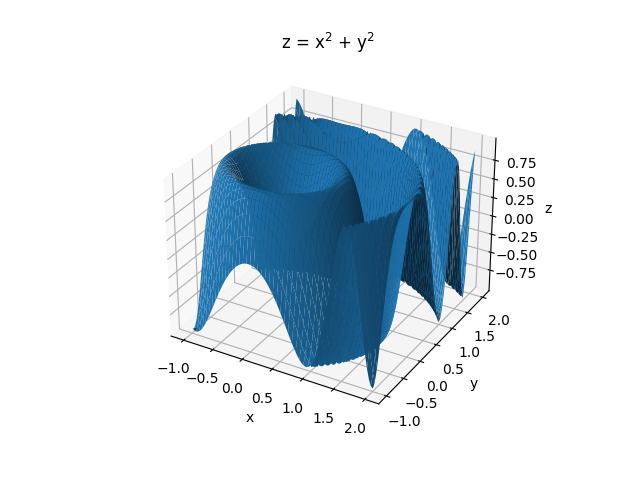
\includegraphics[width=0.8\columnwidth]{3dgraph.png}\label{fig:graph2}}
\label{fig:graphs}
\end{figure}


Figure ~\ref{fig:graph2} shows the equation of the wave:\begin{equation}z = sin(2x^2+3y^2)\end{equation}
Here, if we see the contour lines in the X-Y plane, we obtain an ellipse of the form $2x^2+3y^2=k$ where $k$ is a constant. The sine of this $k$ value is represented on the z-axis.The domain of Z is always positive since the $x$ and $y$ terms are squared. Thus the values for Z lie from $z=0$ to $z=1$ since that is the range of the sine function.
\end{document}